\section{Surprising features in Python}
When working so close to the specification of a language some weird or surprising structures in the language arise.
While we programmed the conversion from abstract syntax tree to a control flow graph, we had these experiences once in a while, and working with the structures has given us some insight, both in the workings of python and in the details of these interesting structures.
This section will discuss some of these experiences.

\subsection{While - else}
Normally we know \texttt{while} as a simple control structure that has a condition and a body.
The body will execute until the condition is false.
This implementation is also found in Python, but Python has an extra variant of the while loop - an else clause.
An example of a while loop with an else clause can be seen on \cref{surprise_while_else}.

\begin{figure}
  \centering
  \begin{subfigure}[b]{0.4\textwidth}
    \begin{lstlisting}[style=python]
while x < threshold:
    if invalid_value(x):
        break
    x += 1
else:
    handle_value()
    \end{lstlisting}
    \caption{A while loop with an else clause}\label{surprise_while_else}
    \end{subfigure}
  ~
    \begin{subfigure}[b]{0.4\textwidth}
      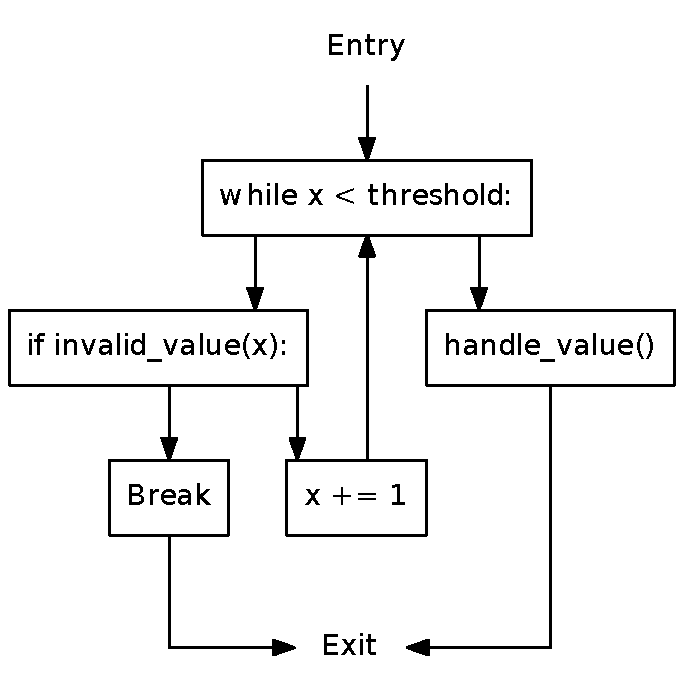
\includegraphics[scale=.5]{./figures/while_break.pdf}
      \caption{Possible flows}\label{surprise_while_else_cfg}
    \end{subfigure}
    
  \caption{An example of a while loop with a break statement}
\end{figure}


The else clause will execute when the condition is false, but if the body is exited by a \texttt{break} statement, the else clause will not be executed.
In the example in \cref{surprise_while_else}, this is being utilised to handle values that are unexpected in some way.
If that is the case, we break the body and do not execute the else clause which contains some logic for the value behaved as expected.

The \texttt{for} loop in Python also has an \texttt{else} clause which works in the same way.
A example of this can be seen in \cref{python:for:else}.

\begin{figure}
  \centering
  \begin{subfigure}[b]{0.4\textwidth}
    \begin{lstlisting}[style=python]
for x in range(5):
    if invalid_value(x):
        break
    print(x)
else:
    print('Accepted')
    \end{lstlisting}
    \caption{Code example}\label{python:for:else:code}
  \end{subfigure}
  ~ %add desired spacing between images, e. g. ~, \quad, \qquad, \hfill etc. 
  %(or a blank line to force the subfigure onto a new line)
  \begin{subfigure}[b]{0.4\textwidth}
    \centering
    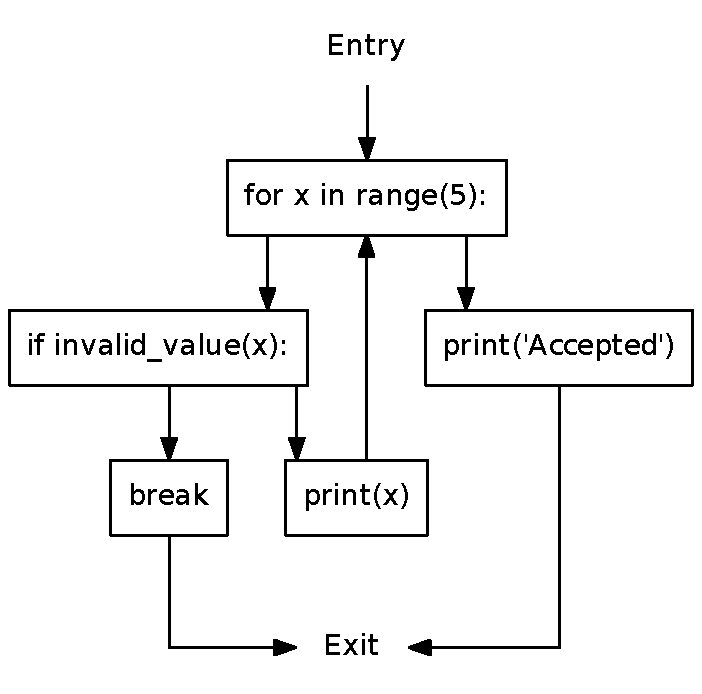
\includegraphics[scale=.5]{./figures/for_else.pdf}
    \caption{Possible flows}
    \label{python:for:else:flow}
  \end{subfigure}
  \caption{A \texttt{for} control structure with an \texttt{else} statement}
  \label{python:for:else}
\end{figure}

\subsection{Generator expression}
The Python language has a goal of being simple, explicit and readable\citep{python_zen}.
This can often be seen in some very elegant constructions contained in the language.
One of those is the generator statement, which was discovered during the development of \pyt{}.

A generator expression is a concise notation for a common pattern: iterating over a collection of items and then performing some operation on every element\citep{python_functional}.

\begin{lstlisting}[style=python, caption={Generator expression, stripping white-space from strings}, label={generator_strip}]
strings = ['King Arthur   ', '', '   Queen Elizabeth',
           '', '   Arnold Schwarzenegger   ']

people = (line.strip() for line in strings if line != '')
\end{lstlisting}

In \cref{generator_strip} some file has been parsed into an array.
The resulting strings have some undesirable white-space, and some of the strings are even empty.
The subsequent generator expression handles both of these problems.

A generator expression consists of an expression part and a for part.
The for part is evaluated and the expression is executed on each element of the resulting iterable.
The result is a generator that contains the results.

In \cref{generator_strip} the generator iterates over the strings with the \texttt{for} statement and filters out empty strings with the \texttt{if} statement.
The resulting elements are the stripped of white-space by the initial expression.

The generator in \cref{generator_strip} can be written without using a generator expression.
This can be seen in \cref{generator_corresponding}.
The generator expression is very clear in conveying its purpose while being shorter than the ``old way''.
\begin{lstlisting}[style=python, caption={\Cref{generator_strip} implemented without using an generator expression}, label={generator_corresponding}]
for line in strings:
    if not line != '':
        yield line.strip()
\end{lstlisting}

Python contains similar constructs called the comprehensions which return a list, set or dictionary of the element instead of a generator.
This construct uses square or curly parenthesis instead of round parenthesis, but are not different in any other way.
An example of a list comprehension can be seen in \cref{listcomp}.

\begin{lstlisting}[style=python, caption={The generator from \cref{generator_strip} changed to a list comprehension}, label={listcomp}]
people = [line.strip() for line in strings if line != '']
\end{lstlisting}

\subsection{Parameter Passing}
This section describes how Python deals with parameter passing and is inspired by \citet{parameter_passing}, official documentation for this can be found at \citet{parameter_passing_official}.
This section is included as we were surprised how it is dealt with and it is important to factor in when parameters are assigned in functions.

The most known parameter passing techniques are pass-by-reference and pass-by-value.
A short description of these two will lead up to an explanation of how Python is handling parameter passing.
To illustrate the different approaches the following two functions are used, \cref{parameter_passing:reassign} and \cref{parameter_passing:append}.

\begin{lstlisting}[style=python, caption={Parameter passing: \texttt{reassign} function.}, label={parameter_passing:reassign}]
  def reassign(l):
      l = [1]
\end{lstlisting}

\begin{lstlisting}[style=python, caption={Parameter passing: \texttt{append} function.}, label={parameter_passing:append}]
  def append(l):
      l.append(1)
\end{lstlisting}

An abstract way of showing the internal representation will be used.
An example can be seen on \cref{parameter_example} where we have a variable \texttt{l} which points at a list which is an object stored in memory as \texttt{[0]}.
In python a variable is just a name that points to some object in memory.
A name is illustrated as a box.
Assigning 1 to a variable and then reassigning it to 2 does not change the 1 in memory.
It just saves the 2 object in memory and makes the variable point at this object.

\ppv{l}{[0]}{A variable \texttt{l} pointing at a list \texttt{[0]}}{parameter_example}

\paragraph{Pass-by-reference}
Pass-by-reference is a parameter passing mechanich where the argument is directly passed into the function.
Consider passign \texttt{l = [0]} to the function \texttt{reassign}.
After the call the object \texttt{l} is changed to: \texttt{l = [1]}, visualised on \cref{parameter_reference_reassign}.

\ppv{l}{[1]}{The variable \texttt{l} pointing at the list \texttt{[0]} after calling function \texttt{reassign}}{parameter_reference_reassign}

This is because the variable is passed directly which means that the function is operating directly on the object.
The \texttt{append} function behaves similarly, but because append adds to the list the result is: \texttt{l = [0, 1]}, visualised in \cref{parameter_reference_append}.

\ppv{l}{[0, 1]}{The variable \texttt{l} pointing at the list \texttt{[0, 1]} after calling function \texttt{append}}{parameter_reference_append}


\paragraph{Pass-by-value}
The other well known parameter passign mechanism is pass-by-value, where the actual parameter is copied and passed into the function.
The actual parameter is copied and stored a new place in memory and the copy is passed into the function.
Given the object \texttt{l = [0]} passed as parameter to the function \texttt{reassign}, the copied object \texttt{l$'$} is changed to: \texttt{l$'$ = [1]}.
The original object \texttt{l}  remains the same as it is not manipulated by the function.

\begin{figure}[H]
  \ppvs{l}{[0]}{The variable \texttt{l} pointing at the list \texttt{[0]} after calling the functions \texttt{reassign}}{parameter_value_l}
  ~
  \ppvs{l$'$}{[1]}{The variable \texttt{l$'$} pointing at the list  \texttt{[1]} after calling function \texttt{reassign}}{parameter_value_lprime}
  \caption{When reassigning in pass-by-value, only the copied list is changed}
\end{figure}

A similar thing happens in the \texttt{append} function, where after calling the function \texttt{l = [0]} and \texttt{l$'$ = [0, 1]}.
To visualise see \cref{parameter_value_l} and \cref{parameter_value_lprime}, here it becomes clear that when we access \texttt{l} after the call nothing has changed.

\begin{figure}[H]
  \ppvs{l}{[0]}{The variable \texttt{l} pointing at the list \texttt{[0]} after calling the functions and \texttt{append}}{parameter_value_l}
  ~
  \ppvs{l$'$}{[0, 1]}{The variable \texttt{l$'$} pointing at the list \texttt{[0, 1]} after calling function \texttt{append}}{parameter_value_lprime}
  \caption{When appending in pass-by-value, only the copied list is changed}
\end{figure}

\paragraph{Pass-by-object-reference}
Pass-by-object-reference is the Python way of handling parameter passing.
In this parameter passing mechanism the argument is copied into a new variable local to the function, but both refer to the same object in memory.
Given the object \texttt{l = [0]} when calling the function \texttt{reassign}, a new variable \texttt{l$'$} is created that refers to the same \texttt{[0]} object in memory.
So \texttt{reassign} sets \texttt{l$'$ = [1]} but not \texttt{l} because \texttt{reassign} is not manipulating the object but only the name that is referring to it.
Calling \texttt{reassign} manipulates the variables and is visualised in \cref{parameter_object_reassign_l} and \cref{parameter_object_reassign_lprime}.

\begin{figure}[H]
  \ppvs{l}{[0]}{The variable \texttt{l} pointing at the list \texttt{[0]} after calling function \texttt{reassign}}{parameter_object_reassign_l}
  ~
  \ppvs{l$'$}{[1]}{The variable \texttt{l$'$} pointing at the list \texttt{[1]} after calling function \texttt{reassign}}{parameter_object_reassign_lprime}
  \caption{Pass-by-object-reference copies the variable, but points it at the same object as the original variable}
\end{figure}

When calling the \texttt{append} function the object is referenced and both \texttt{l} and \texttt{l$'$} are changed to \texttt{[0, 1]}.
Calling \texttt{append} manipulates the objects referenced by the variables.
This is visualised in \cref{parameter_object_append}.

\begin{figure}[h]
   \centering
\begin{tikzpicture}
  \node[draw, line width=0.05mm, minimum width=1cm,minimum height=1cm, outer sep=10pt] (mem1) at (1.75,5) {l};
  \node[draw, line width=0.05mm, minimum width=1cm,minimum height=1cm, outer sep=10pt] (mem2) at (1.75,3) {l$'$};  
  \node (result) at (3.5,4) {[0, 1]};
  \draw[<-] (result) -- (mem1);
  \draw[<-] (result) -- (mem2);
\end{tikzpicture}   
  \caption{The variable \texttt{l} and \texttt{l$'$} stored in memory as \texttt{[0, 1]} when calling function \cref{parameter_passing:append}.}
  \label{parameter_object_append}
\end{figure}
